\documentclass[11pt]{article}

\usepackage[margin=1in]{geometry}
\usepackage{booktabs}
\usepackage{tabularx}
\usepackage[hidelinks]{hyperref}
\usepackage{parskip}
\usepackage{enumitem}
\usepackage{verbatim}
\usepackage{tikz}
\usepackage{pgfplots}
\usetikzlibrary{arrows.meta,positioning,shapes.geometric,calc}
\pgfplotsset{compat=1.18}

\setlist{nosep}
\setcounter{tocdepth}{2}
\setlength{\emergencystretch}{2em}
\newcommand{\iface}[5]{#1\par\begin{quote}\small\ttfamily\raggedright #2\par\end{quote}
\begin{tabularx}{\textwidth}{@{}p{.24\textwidth}p{.21\textwidth}Xp{.12\textwidth}@{}}\toprule Name & Shape/type & Meaning & Units \\\midrule #3\\\bottomrule\end{tabularx}
\begin{tabularx}{\textwidth}{@{}p{.30\textwidth}X@{}}\toprule Output & Meaning \\\midrule #4\\\bottomrule\end{tabularx}
\begingroup\sloppy #5\par\endgroup\medskip}

\begin{document}

\begin{center}
    {\LARGE\bfseries Design Document: BMTP Motion-Generation Engine
    (\texttt{trajectory/+bmtpEngine})\par}
    \vspace{1.5em}
    \begin{tabular}{@{}ll@{}}
        \textbf{Author:} & Kevin Trinh \\
        \textbf{Status:} & Draft \\
        \textbf{Last updated:} & 2026-08-31 \\
        \textbf{Reviewers:} & TBD
    \end{tabular}
\end{center}

\tableofcontents
\newpage

\section{Context}

The repository provides one public obstacle-avoidance planner in the
azimuth/elevation frame. The planner owns obstacle interpretation, topology
search, candidate selection, and authoritative validation. It delegates all
motion generation to a separate engine, \texttt{trajectory/+bmtpEngine}.

The engine is dimension-neutral. It does not import obstacle or planner
packages. It receives only numeric inputs: a topology seed, finite convex
exclusion polygons, normalized endpoint states, and normalized limits. This
boundary lets the planner change its geometry pipeline without an engine
change, and lets tests exercise the engine in isolation.

Position uses degrees. Time uses seconds. Derivatives use deg/s,
deg/s$^2$, and deg/s$^3$.

\section{Goals}

\begin{itemize}
    \item Generate exact minimum-time synchronized rest-to-rest motion with analytic
    jerk-switching laws and lossless time scaling.
    \item Optimize one static topology seed with a composite Bezier trajectory,
    third-order time-power cones, and alternating degree-one maximum-margin
    separating planes (the BMTP solve).
    \item Accept a motion only after direct Bernstein checks and an all-span,
    all-region separating-plane certificate.
    \item Return stable diagnostics for every outcome, including expected
    infeasibility, work-limit stops, and stagnation stops.
    \item Provide exact supporting constructions: dwell prepend, quintic coordinate
    offsets, lateral progress composition, and event-word integration.
\end{itemize}

\section{Non-goals}

\begin{itemize}
    \item Obstacle interpretation. The planner converts protected geometry to numeric
    convex exclusion regions before any engine call.
    \item Authoritative acceptance. The public validator remains the final authority
    for coverage, continuous collision freedom, workspace, endpoints, and
    derivative limits.
    \item Global optimality proofs. A validated candidate is a feasible incumbent
    unless a request-wide physical lower certificate applies.
    \item Dynamic obstacle families. Cavity, timed-opening, and fixed-clock lateral
    constructions stay planner-owned because they interpret geometry and timing.
\end{itemize}

\section{Overview}

\begin{verbatim}
planner (obstacleAvoidance)                engine (+bmtpEngine)
---------------------------                ---------------------
seed, convex regions, states,   ------>    solve
limits, options, warm start                  1. validate; build static
                                                Bezier representation
                                             2. alternate time-power SOCP
                                                and max-margin plane SOCP
                                             3. project, dilate, certify
                                             4. finalize candidate record
candidate, diagnostics,        <------
restart (certified net)
\end{verbatim}

Obstacle-free rest-to-rest requests bypass the SOCP path. They use the exact
synchronized switching kernel (\texttt{createDirectMotion}). Fixed arrival times
stretch the same law without increasing any derivative.

Figure~\ref{fig:boundary} replaces the earlier text diagram. A topology seed is
a route-shaped point list. A separating plane is a line that puts a curve span
and a convex exclusion region on opposite sides.
\begin{figure}[ht]\centering
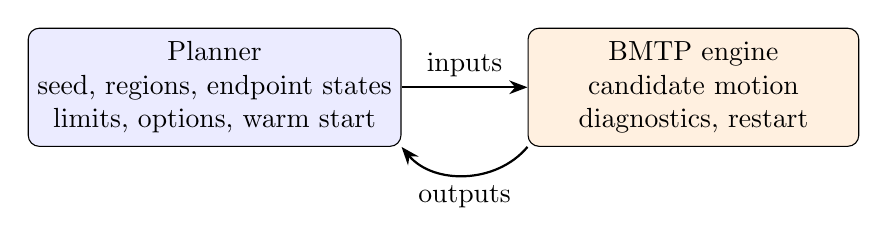
\begin{tikzpicture}[node distance=16mm,box/.style={draw,rounded corners,align=center,minimum width=42mm,minimum height=15mm},->,>=Stealth]
\node[box,fill=blue!8](p){Planner\\seed, regions, endpoint states\\limits, options, warm start};
\node[box,fill=orange!12,right=of p](e){BMTP engine\\candidate motion\\diagnostics, restart};
\draw[->,thick](p)--node[above]{inputs}(e);
\draw[->,thick](e.south west)to[out=230,in=310]node[below]{outputs}(p.south east);
\end{tikzpicture}
\caption{Boundary between obstacle avoidance and the engine.}\label{fig:boundary}
\end{figure}

Figure~\ref{fig:solveflow} shows \texttt{solve}. The time-power SOCP is a
convex program that applies derivative limits while duration is a variable.
\begin{figure}[ht]\centering
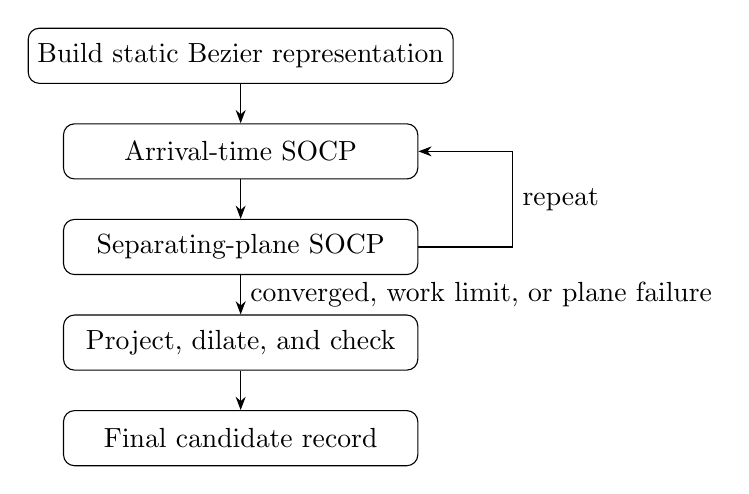
\begin{tikzpicture}[node distance=5mm,box/.style={draw,rounded corners,align=center,minimum width=45mm,minimum height=7mm},->,>=Stealth]
\node[box](a){Build static Bezier representation};\node[box,below=of a](b){Arrival-time SOCP};\node[box,below=of b](c){Separating-plane SOCP};\node[box,below=of c](d){Project, dilate, and check};\node[box,below=of d](f){Final candidate record};
\draw[->](a)--(b);\draw[->](b)--(c);\draw[->](c.east)--++(12mm,0)|-node[pos=.25,right]{repeat}(b.east);\draw[->](c)--node[right]{converged, work limit, or plane failure}(d);\draw[->](d)--(f);
\end{tikzpicture}
\caption{The alternating BMTP solve and its three stopping outcomes.}\label{fig:solveflow}
\end{figure}

Figure~\ref{fig:warmstart} shows the warm-start path. Bernstein form expresses
a polynomial by control points. Its convex-hull property bounds a full span,
not only sampled points.
\begin{figure}[ht]\centering
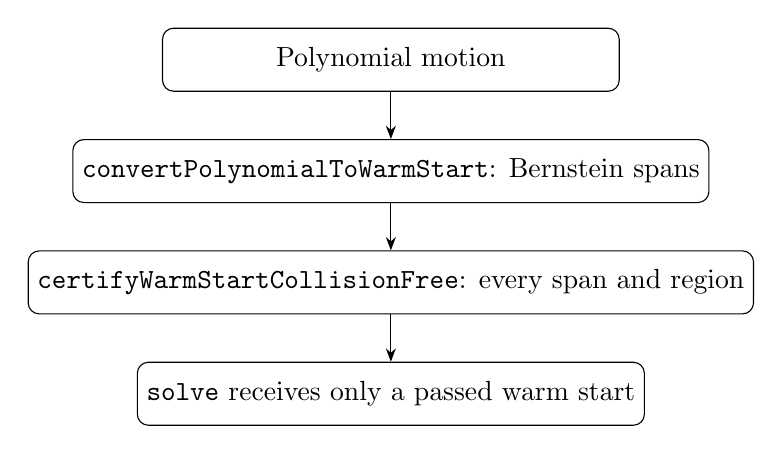
\begin{tikzpicture}[node distance=6mm,box/.style={draw,rounded corners,align=center,minimum width=58mm,minimum height=8mm},->,>=Stealth]
\node[box](a){Polynomial motion};\node[box,below=of a](b){\texttt{convertPolynomialToWarmStart}: Bernstein spans};\node[box,below=of b](c){\texttt{certifyWarmStartCollisionFree}: every span and region};\node[box,below=of c](d){\texttt{solve} receives only a passed warm start};
\draw[->](a)--(b);\draw[->](b)--(c);\draw[->](c)--(d);
\end{tikzpicture}
\caption{Warm-start approximation and collision certification.}\label{fig:warmstart}
\end{figure}

\section{Detailed design}

\subsection{Public surface}

\small
\begin{tabularx}{\textwidth}{@{}>{\ttfamily\raggedright\arraybackslash}p{0.35\textwidth}X@{}}
\toprule
\normalfont Function & Responsibility \\
\midrule
solve & Optimize one static seed; return candidate, diagnostics, restart. \\
createDirectMotion & Exact minimum-time synchronized rest-to-rest motion. \\
createDelayedMotion & Prepend a stationary dwell; repartition an exact cubic motion. \\
createOffsetSplineMotion & Add a minimum-integrated-jerk quintic offset to one coordinate. \\
createProgressPolynomialMotion & Compose an endpoint-flat lateral path over one straight progress motion. \\
createMotionRecord & Build the shared candidate record; integrate a piecewise-constant-jerk event word exactly. \\
createCoordinateTolerances & Derive one coordinate scale and the shared geometric tolerances. \\
evaluatePolynomial & Evaluate ascending-power segment records at absolute times. \\
maximumRestToRestDistance & Exact maximum scalar displacement in one clock. \\
convertPolynomialToWarmStart & Approximate a piecewise polynomial with equal-duration Bernstein spans. \\
certifyWarmStartCollisionFree & Certify every warm-start span against every region before BMTP. \\
\bottomrule
\end{tabularx}
\normalsize

\subsection{What the planner provides and what the engine returns}

\begin{itemize}
    \item \textbf{Seed.} \texttt{position\_deg} is N-by-2. \texttt{tau} strictly increases from zero to
    one.
    \item \textbf{Regions.} An R-by-1 cell array. Each cell holds one finite convex N-by-2
    exclusion polygon in degrees. Plane witnesses certify only these supplied
    regions.
    \item \textbf{Coverage.} A planner-owned proof record. The engine requires
    \texttt{Passed}. When the \texttt{Applied} field in
    \texttt{ConservativeGrouping} is true, the solve uses the compact
    degree-7 representation with one split; otherwise it uses the default
    representation.
    \item \textbf{Warm start.} A previously certified
    \texttt{ControlPoint\_deg} array and \texttt{SegmentTime\_s}.
    \texttt{certifyWarmStart\allowbreak CollisionFree} must pass before entering
    the SOCP loop.
    \item \textbf{Candidate.} One stable motion record shared by all construction paths.
    Expected infeasibility returns \texttt{Success=false} with preserved diagnostics.
    \item \textbf{Restart.} The certified parent control net and segment time, returned for
    exact later refinement.
\end{itemize}

\subsection{The BMTP solve loop}

\texttt{solve} alternates two convex programs over a composite Bezier curve:

\begin{enumerate}
    \item \textbf{Time-power SOCP.} Third-order time-power cones minimize arrival time
    subject to derivative limits, endpoint conditions, and the current
    separating planes.
    \item \textbf{Maximum-margin plane SOCP.} Degree-one Bernstein separating planes are
    re-derived for every span/region pair to maximize clearance margin.
\end{enumerate}

The loop stops on convergence, on the work limit, or on the stagnation
stop. The immutable conic structure (derivative, endpoint, and continuity
matrices; equality right-hand side; objective; bound template; second-order
cones) is cached per seed. Plane-dependent rows and the active horizon bound
are rebuilt on every alternation in the original order.

\subsection{Certification before acceptance}

Acceptance requires all of the following, in order:

\begin{enumerate}
    \item Direct Bernstein checks on the selected motion. Segment-local power
    coefficients are converted to Bernstein form. The convex-hull property
    bounds complete polynomial intervals; the engine does not rely on sampled
    points alone.
    \item An all-span, all-region degree-one plane certificate after projection and
    dilation.
    \item Independent public validation by the planner-side validator. The engine
    never self-certifies a final result.
\end{enumerate}

Figure~\ref{fig:geometry} shows the geometric test. Clearance is the certified
distance between the span and the region.
\begin{figure}[ht]\centering
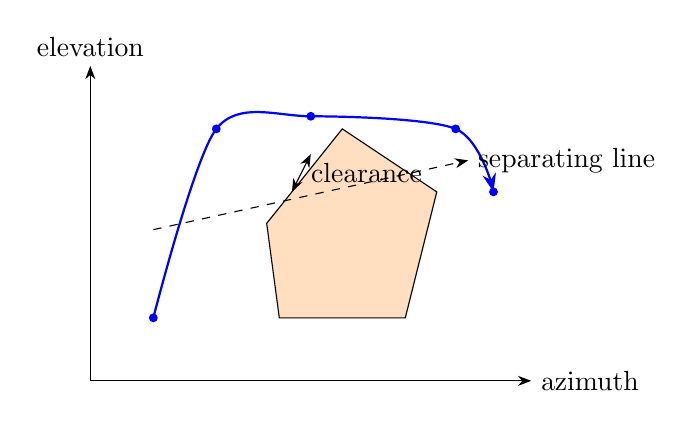
\begin{tikzpicture}[scale=.8,->,>=Stealth]
\draw[->](0,0)--(7,0)node[right]{azimuth};\draw[->](0,0)--(0,5)node[above]{elevation};
\filldraw[fill=orange!25](3,1)--(5,1)--(5.5,3)--(4,4)--(2.8,2.5)--cycle;
\draw[blue,thick]plot[smooth]coordinates{(1,1)(2,4)(3.5,4.2)(5.8,4)(6.4,3)};
\foreach \p in {(1,1),(2,4),(3.5,4.2),(5.8,4),(6.4,3)}\fill[blue]\p circle(2pt);
\draw[dashed](1,2.4)--(6,3.5)node[right]{separating line};
\draw[<->](3.2,3)--(3.5,3.6)node[midway,right]{clearance};
\end{tikzpicture}
\caption{A polygon, a composite Bezier path, and a separating line.}\label{fig:geometry}
\end{figure}

Figure~\ref{fig:builders} relates the exact motion builders.
\begin{figure}[ht]\centering
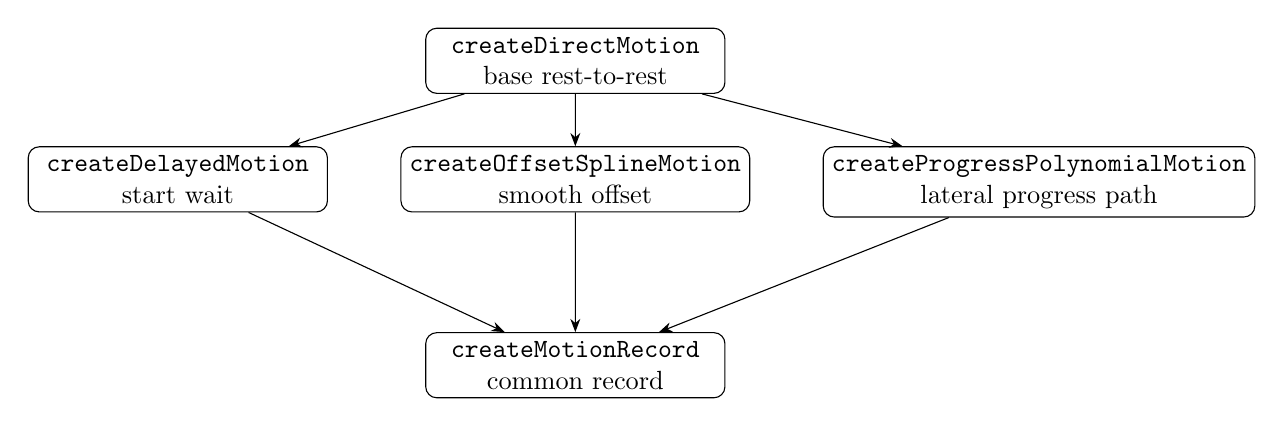
\begin{tikzpicture}[scale=.95,transform shape,node distance=7mm and 13mm,box/.style={draw,rounded corners,align=center,minimum width=40mm,minimum height=8mm},->,>=Stealth]
\node[box](a){\texttt{createDirectMotion}\\base rest-to-rest};
\node[box,below left=of a](b){\texttt{createDelayedMotion}\\start wait};
\node[box,below=of a](c){\texttt{createOffsetSplineMotion}\\smooth offset};
\node[box,below right=of a](d){\texttt{createProgressPolynomialMotion}\\lateral progress path};
\node[box,below=16mm of c](e){\texttt{createMotionRecord}\\common record};
\draw[->](a)--(b);\draw[->](a)--(c);\draw[->](a)--(d);\draw[->](b)--(e);\draw[->](c)--(e);\draw[->](d)--(e);
\end{tikzpicture}
\caption{How exact motion builders create a common candidate record.}\label{fig:builders}
\end{figure}

\section{Public interface reference}
\subsection{\texttt{solve}}
\iface{Optimizes one static topology seed. The planner calls it after it has
created convex exclusion regions and normalized the request.}
{[candidate, diagnostics, restart] =\allowbreak{} bmtpEngine.solve(seed,\allowbreak{}
regions\_deg,\allowbreak{} coverage,\allowbreak{} initialState,\allowbreak{}
goalState,\allowbreak{} limits,\allowbreak{} options,\allowbreak{} warmStart)}
{\texttt{seed} & scalar struct & N-by-2 route and increasing \texttt{tau} & degrees \\
\texttt{regions\_deg} & R-by-1 cell array & convex exclusion polygons & degrees \\
\texttt{coverage} & scalar struct & planner coverage proof with \texttt{Passed} & -- \\
\texttt{initialState}, \texttt{goalState} & scalar structs & rest endpoints and times & degrees, seconds \\
\texttt{limits}, \texttt{options} & scalar structs & bounds, time policy, work limits & mixed \\
\texttt{warmStart} & scalar struct or empty & certified control net and span time & degrees, seconds}
{\texttt{candidate} & stable motion record \\
\texttt{diagnostics} & solver, timing, coverage, and certificate evidence \\
\texttt{restart} & parent control net and segment time}
{Invalid inputs and malformed warm starts raise errors. Expected infeasibility
returns \texttt{Success=false}, including no feasible iterate, an infeasible
time window, or an unavailable plane certificate.}

\subsection{\texttt{createDirectMotion}}
\iface{Creates exact synchronized rest-to-rest motion. The planner calls it for
a direct request and as a base for later composition.}
{candidate =\allowbreak{} bmtpEngine.createDirectMotion(initialState,\allowbreak{}
goalState,\allowbreak{} limits,\allowbreak{} options)}
{\texttt{initialState}, \texttt{goalState} & scalar structs & time, position, optional rest derivatives & degrees, seconds \\
\texttt{limits} & scalar struct & positive velocity, acceleration, jerk bounds & derivative units \\
\texttt{options} & scalar struct & goal-time mode, sample time, tolerance & seconds, degrees}
{\texttt{candidate} & stable exact polynomial and sampled-motion record}
{Invalid states, limits, options, and time horizons raise errors. Unsupported
endpoint derivatives, zero displacement, too-short arrival, and reconstruction
failure return \texttt{Success=false}.}

\subsection{\texttt{createDelayedMotion}}
\iface{Adds a stationary dwell before an existing cubic motion. The planner
calls it when a wait must keep the exact base motion.}
{candidate =\allowbreak{} bmtpEngine.createDelayedMotion(baseMotion,\allowbreak{}
initialState,\allowbreak{} breakTime\_s,\allowbreak{} sampleStep\_s,\allowbreak{}
seedSource)}
{\texttt{baseMotion} & scalar result struct & complete cubic polynomial & -- \\
\texttt{initialState} & scalar struct & start state & degrees, seconds \\
\texttt{breakTime\_s} & numeric vector & increasing absolute break times & seconds \\
\texttt{sampleStep\_s}, \texttt{seedSource} & scalar, scalar text & history spacing and source label & seconds, --}
{\texttt{candidate} & exact delayed polynomial and histories}
{Invalid calls, degree, partition, sampling, and labels raise errors. A valid
request has no separate normal failure record.}

\subsection{\texttt{createOffsetSplineMotion}}
\iface{Adds a smooth scalar offset to one coordinate. The planner calls it when
offset knots define a lateral change. It uses a minimum-integrated-jerk quintic
spline, which minimizes the integral of jerk squared.}
{candidate =\allowbreak{} bmtpEngine.createOffsetSplineMotion(baseMotion,\allowbreak{}
knotTime\_s,\allowbreak{} knotOffset\_deg,\allowbreak{} axisIndex,\allowbreak{}
initialState,\allowbreak{} sampleStep\_s,\allowbreak{} seedSource)}
{\texttt{baseMotion} & scalar result struct & complete base polynomial & -- \\
\texttt{knotTime\_s}, \texttt{knotOffset\_deg} & matching vectors & increasing offset knots & seconds, degrees \\
\texttt{axisIndex} & positive integer & offset coordinate & -- \\
\texttt{initialState}, \texttt{sampleStep\_s}, \texttt{seedSource} & struct, scalar, text & state, spacing, label & mixed}
{\texttt{candidate} & composite polynomial and sampled histories}
{Invalid calls, knots, axes, clock ends, sampling, and labels raise errors. A
valid construction returns a motion record.}

\subsection{\texttt{createProgressPolynomialMotion}}
\iface{Layers an endpoint-flat lateral path over a straight-progress motion.
Endpoint-flat means the added path and its endpoint derivatives vanish.}
{candidate =\allowbreak{} bmtpEngine.createProgressPolynomialMotion(baseMotion,\allowbreak{}
initialState,\allowbreak{} goalState,\allowbreak{} progressAxisIndex,\allowbreak{}
amplitude\_deg,\allowbreak{} sampleStep\_s,\allowbreak{} seedSource)}
{\texttt{baseMotion} & scalar result struct & successful two-coordinate straight progress & -- \\
\texttt{initialState}, \texttt{goalState} & scalar structs & two-coordinate rest endpoints & degrees, seconds \\
\texttt{progressAxisIndex}, \texttt{amplitude\_deg} & integer, scalar & progress coordinate and lateral coefficient & --, degrees \\
\texttt{sampleStep\_s}, \texttt{seedSource} & scalar, text & spacing and label & seconds, --}
{\texttt{candidate} & exact degree-15 composed motion}
{Invalid base motion, endpoints, axes, zero progress, or labels raise errors.
A valid construction returns a motion record.}

\subsection{\texttt{createMotionRecord}}
\iface{Creates the common candidate record. Builders call it to integrate an
event word exactly. An event word is time breaks with constant jerk per
interval. It can also package an assembled polynomial.}
{[candidate, terminalState] =\allowbreak{}
bmtpEngine.createMotionRecord(candidate,\allowbreak{} initialState,\allowbreak{}
relativeBreak\_s,\allowbreak{} segmentJerk\_deg\_s3,\allowbreak{}
sampleStep\_s,\allowbreak{} seedSource)}
{\texttt{candidate} & scalar struct & empty creates the common record & -- \\
\texttt{initialState} & scalar struct & position, velocity, acceleration & derivative units \\
\texttt{relativeBreak\_s} & vector, polynomial, or empty & event breaks or polynomial & seconds \\
\texttt{segmentJerk\_deg\_s3} & N-by-D numeric & constant interval jerk & degrees per second cubed \\
\texttt{sampleStep\_s}, \texttt{seedSource} & scalar, text & spacing and label & seconds, --}
{\texttt{candidate} & stable polynomial and history record \\
\texttt{terminalState} & exact terminal state}
{Empty breaks return the stable not-run record. Invalid polynomials and event
words raise errors.}

\subsection{\texttt{createCoordinateTolerances}}
\iface{Derives one coordinate scale and shared geometric tolerances. The engine
uses it where construction and collision checks need the same roundoff
allowance. A roundoff reserve is an allowance for finite precision.}
{[coordinateScale\_deg, geometryTolerance\_deg, roundoffReserve\_deg]
=\allowbreak{} bmtpEngine.createCoordinateTolerances(values\_deg,\allowbreak{} ...)}
{\texttt{values\_deg} & numeric arrays or cells & coordinate collections; nonfinite values ignored & degrees}
{\texttt{coordinateScale\_deg} & maximum finite absolute coordinate, at least one degree \\
\texttt{geometryTolerance\_deg} & shared geometric tolerance \\
\texttt{roundoffReserve\_deg} & conservative finite-precision reserve}
{Nonnumeric coordinate collections raise errors. Valid calls always return
tolerances and have no failure record.}

\subsection{\texttt{evaluatePolynomial}}
\iface{Evaluates common ascending-power polynomial records at absolute times.
Ascending power means coefficients start with the constant term. The engine
uses it for histories and warm-start comparisons.}
{[time\_s, position\_deg, velocity\_deg\_s, acceleration\_deg\_s2,
jerk\_deg\_s3] =\allowbreak{} bmtpEngine.evaluatePolynomial(polynomial,\allowbreak{}
time\_s,\allowbreak{} segmentIndex)}
{\texttt{polynomial} & scalar struct & N-by-D-by-P ascending-power records & derivative units \\
\texttt{time\_s} & numeric vector & absolute request times & seconds \\
\texttt{segmentIndex} & scalar or vector, optional & exact segment selection & --}
{\texttt{time\_s} & normalized N-by-1 time column \\
\texttt{position\_deg} through \texttt{jerk\_deg\_s3} & N-by-D histories}
{Empty or nonfinite times return NaN histories. Malformed polynomial data and
incompatible indices raise ordinary MATLAB errors.}

\subsection{\texttt{maximumRestToRestDistance}}
\iface{Returns the exact maximum scalar rest-to-rest displacement for one clock.
It uses the same jerk-limited, acceleration-limited, and velocity-limited
switching regimes as the direct builder.}
{distance\_deg =\allowbreak{}
bmtpEngine.maximumRestToRestDistance(duration\_s,\allowbreak{}
velocityLimit\_deg\_s,\allowbreak{} accelerationLimit\_deg\_s2,\allowbreak{}
jerkLimit\_deg\_s3)}
{\texttt{duration\_s} & nonnegative scalar & available motion duration & seconds \\
\texttt{velocityLimit\_deg\_s} & positive scalar & symmetric velocity limit & degrees per second \\
\texttt{accelerationLimit\allowbreak\_deg\_s2} & positive scalar & symmetric acceleration limit & degrees per second squared \\
\texttt{jerkLimit\_deg\_s3} & positive scalar & symmetric jerk limit & degrees per second cubed}
{\texttt{distance\_deg} & exact maximum displacement}
{Invalid duration or limits raise errors. Valid calls return a nonnegative
distance.}

\subsection{\texttt{convertPolynomialToWarmStart}}
\iface{Approximates a piecewise polynomial by equal-duration Bernstein spans.
The planner calls it before warm-start certification. It measures error but
does not approve the approximation.}
{[warmStart, diagnostics] =\allowbreak{}
bmtpEngine.convertPolynomialToWarmStart(polynomial,\allowbreak{}
segmentCount,\allowbreak{} degree)}
{\texttt{polynomial} & scalar struct & source segments with local powers & degrees, seconds \\
\texttt{segmentCount} & positive integer & output span count & -- \\
\texttt{degree} & positive integer & fitted Bernstein degree & --}
{\texttt{warmStart} & control points and common span time \\
\texttt{diagnostics} & fit and check counts and sampled deviations}
{Invalid polynomial records, span counts, and degrees raise errors. A valid
conversion returns an approximation even if its measured error is large.}

\subsection{\texttt{certifyWarmStartCollisionFree}}
\iface{Checks every Bernstein warm-start span against every exclusion region.
It tries a constant separator, then the degree-one separating-plane form. The
planner calls it before it passes a warm start to \texttt{solve}.}
{certificate =\allowbreak{}
bmtpEngine.certifyWarmStartCollisionFree(warmStart,\allowbreak{}
regions\_deg,\allowbreak{} collisionClearanceTolerance\_deg)}
{\texttt{warmStart} & scalar struct & control points and positive span time & degrees, seconds \\
\texttt{regions\_deg} & cell vector & finite convex protected polygons & degrees \\
\texttt{collisionClearance\allowbreak Tolerance\_deg} & nonnegative scalar & required separation after reserve & degrees}
{\texttt{certificate} & all-pair result, planes, reasons, counts, minimum clearance}
{Invalid inputs raise errors. An uncertified warm start returns a failure
record with \texttt{Passed=false} and reason
\texttt{uncertifiedWarmStartCollision}.}

\section{Alternatives considered}

\begin{itemize}
    \item \textbf{Rebuild the full SOCP every alternation (previous behavior).} Rejected
    for cost. Profiling showed the immutable conic structure was rebuilt
    unchanged. The retained cache improved the maintained Target Exits median
    wall time by 9.82\% and the diagnostic mode by 15.34\%, with bit-identical
    reference example results (see \texttt{verification.md}).
    \item \textbf{Separating-plane reuse across alternations.} Rejected. The
    experiment changed accepted results without a controlling bound. The
    restored version is off unless the planner sets \texttt{EnablePlaneReuse} to true, with a
    retained-best improvement bound; the default path preserves the plane reset
    and re-derivation exactly (see \texttt{branch\_assessment.md}).
    \item \textbf{Sample-based collision checking.} Rejected. Sampling cannot bound a full
    polynomial interval. Bernstein convex-hull bounds certify complete spans.
    \item \textbf{Engine-side obstacle interpretation.} Rejected. It would couple the
    engine to planner geometry and break dimension neutrality.
\end{itemize}

\section{Testing, performance, and failure reporting}

\begin{itemize}
    \item \textbf{Testing.} The clean MATLAB suite checks every change (currently 98/98).
    Default reference example cases must remain bit-identical for any change that claims
    no behavior difference. Changed files must be Code Analyzer clean.
    \item \textbf{Performance.} \texttt{coneprog} calls dominate solve cost. Timing claims use
    isolated MATLAB preference snapshots, one discarded warm-up, and interleaved
    A/B repetitions.
    \item \textbf{Failure visibility.} Work limits, exhausted alternation, unsupported
    requests, and physical infeasibility return stable failure records. The
    engine does not throw for expected infeasibility.
\end{itemize}

Figure~\ref{fig:timing} plots measured median wall times from the dated BMTP
immutable SOCP cache section of \texttt{verification.md}. The values are
measured baseline and candidate medians for the four timed cases.
\begin{figure}[ht]\centering
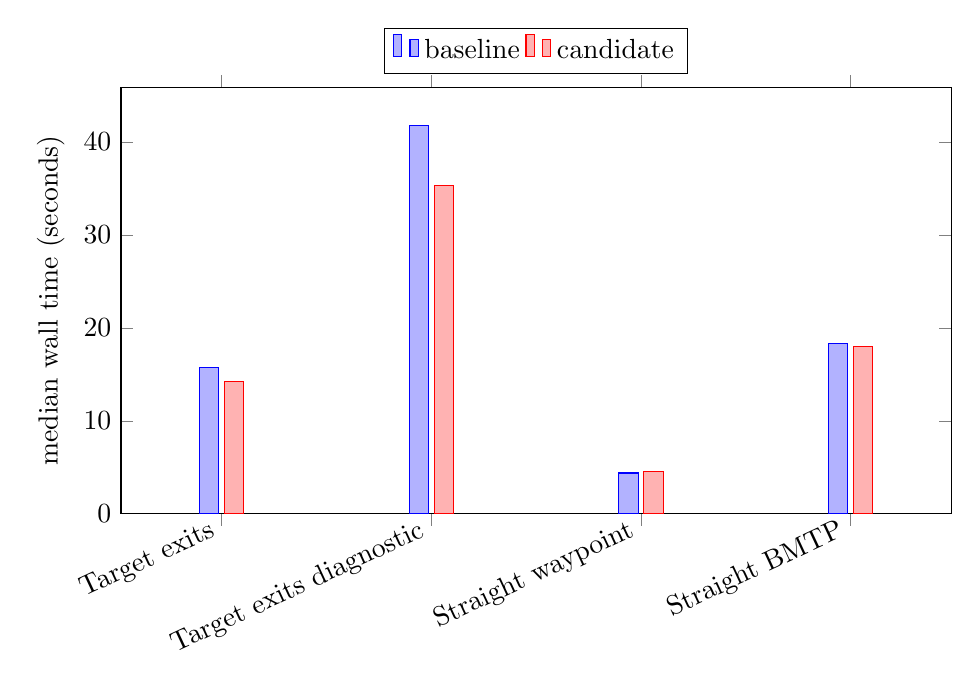
\begin{tikzpicture}
\begin{axis}[ybar,bar width=7pt,width=\textwidth,height=7cm,
ylabel={median wall time (seconds)},ymin=0,
symbolic x coords={Target exits,Target exits diagnostic,Straight waypoint,Straight BMTP},
xtick=data,x tick label style={rotate=25,anchor=east},
legend style={at={(.5,1.03)},anchor=south,legend columns=-1},enlarge x limits=.16]
\addplot coordinates {(Target exits,15.7403272) (Target exits diagnostic,41.7338001) (Straight waypoint,4.3850744) (Straight BMTP,18.3498866)};
\addplot coordinates {(Target exits,14.1946827) (Target exits diagnostic,35.3340565) (Straight waypoint,4.5019727) (Straight BMTP,18.0195969)};
\legend{baseline,candidate}
\end{axis}
\end{tikzpicture}
\caption{Measured median wall times from \texttt{verification.md}. Each pair
compares the recorded baseline and candidate medians for one timed case.}
\label{fig:timing}
\end{figure}

\section{Open questions}

\begin{itemize}
    \item Should the stagnation stop and \texttt{EnablePlaneReuse} controls merge into one
    alternation-policy option?
    \item Can the warm-start position-error bound from \texttt{convertPolynomialToWarmStart}
    feed the dilation margin directly, instead of a fixed tolerance?
    \item Is a request-wide lower-bound certificate practical for seeded BMTP solves,
    so more results can claim bounded arrival instead of incumbent status?
\end{itemize}

\end{document}
